\addchap[Appendix B:$\quad$Graphing with Gnuplot]{Appendix B}
\textsf{\textbf{\Large Graphing with Gnuplot}}\vspace{4mm}

Gnuplot is a free, open-source software package for producing a variety of graphs. Versions are
available for many operating systems. Below is a very brief tutorial on how to use Gnuplot to graph
trigonometric functions.\vspace{4mm}

\par\noindent\textbf{\textsf{INSTALLATION}}
\begin{enumerate}
 \item Go to \url{http://www.gnuplot.info/download.html} and follow the links to download the latest
  version for your operating system. For Windows, you should download the setup file with a name
  such as \path{gp460-win32-setup.exe}, which is
  version 4.6.0. All the examples discussed here will assume at least version 4.6.0, though they
  should work with earlier 4.x versions.
 \item Install the downloaded file. For example, in Windows you would run the setup file you
  downloaded in Step 1, which installs Gnuplot in the
  \texttt{C:\symbol{92}Program Files\symbol{92}gnuplot} folder by default.
  You can accept the defaults during installation, though you
  should select the  ``Create a desktop icon'' option in the \textbf{Select Additional Tasks}
  screen.
 \item (Optional) Read the documentation at \url{http://gnuplot.info/documentation.html}.
\end{enumerate}

\par\noindent\textbf{\textsf{RUNNING GNUPLOT}}
\begin{enumerate}
 \item In Windows, run \textbf{\path{wgnuplot.exe}} from the \path{bin} folder where you
  installed Gnuplot (the default location is
  \texttt{C:\symbol{92}Program Files\symbol{92}gnuplot\symbol{92}bin\symbol{92}wgnuplot.exe}),
  or double-click the desktop icon if you selected that option during the installation.
  In Linux, just type \textbf{\path{gnuplot}} in a terminal window.
 \item You should now get a Gnuplot terminal with a \textbf{\path{gnuplot>}} command prompt. In
  Windows this will appear in a new window, as shown in the picture on the next page.
  In Linux it will appear in the terminal window
  where the \textbf{\path{gnuplot}} command was
  run. For Windows, if the font is unreadable you can change it by right-clicking on the text part
  of the Gnuplot window
  and selecting the ``Choose Font..'' option. For example, the font ``Courier'', style ``Regular'',
  size ``12'' is usually a
  good choice (that choice can be saved for future sessions by right-clicking in the Gnuplot window
  again and selecting the option to update wgnuplot.ini).
 \item At the \textbf{\path{gnuplot>}} command prompt you can now run graphing commands, which we
  will now describe.
\end{enumerate}
\newpage
\begin{figure}[h]
 \begin{center}
  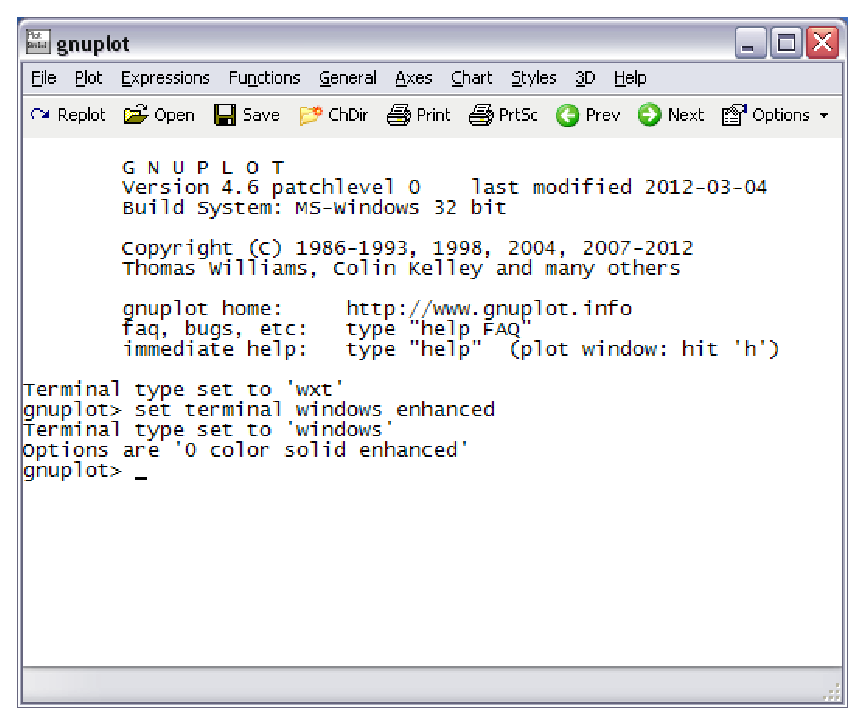
\includegraphics{wgnuplot.eps}
 \end{center}
\end{figure}

\par\noindent\textbf{\textsf{GRAPHING FUNCTIONS}}\vspace{2mm}\\
The usual way to create graphs in Gnuplot is with the \textbf{\path{plot}} command:
\begin{displaymath}
 \texttt{plot \emph{<range> <comma-separated list of functions>}}
\end{displaymath}
For a function $y=f(x)$, \texttt{\emph{<range>}} is the range of $x$ values (and optionally the
range of $y$ values) over which to plot. To specify an $x$ range, use an expression of the form
\symbol{91}$a:b$\symbol{93}, for some numbers $a<b$. This will cause the graph to
be plotted for $a\le x\le b$.\vspace{2mm}

To specify an $x$ range and a $y$ range, use an expression of the form
\symbol{91}$a:b$\symbol{93}\symbol{91}$c:d$\symbol{93}, for some numbers $a<b$ and $c<d$. This will
cause the graph to be plotted for $a\le x\le b$ and $c\le y \le d$.\vspace{2mm}

\par\noindent Function definitions use the $x$ variable in combination with mathematical operators,
listed below:\vspace{1mm}

\begin{center}
\begin{tabular}{@{} | c | c | c | c | @{}}
 \hline \textbf{Symbol} & \textbf{Operation} & \textbf{Example} & \textbf{Result}\\
 \hline $+$ & Addition & $2 + 3$ & $5$\\
 \hline $-$ & Subtraction & $3 - 2$ & $1$\\
 \hline * & Multiplication & $2$*$3$ & $6$\\
 \hline $/$ & Division & $4/2$ & $2$\\
 \hline ** & Power & $2$**$3$ & $2^3 = 8$\\
 \hline exp($x$) & $e^x$ & exp($2$) & $e^2$\\
 \hline log($x$) & $\ln x$ & log($2$) & $\ln 2$\\
 \hline sin($x$) & $\sin x$ & sin(pi/$2$) & $1$\\
 \hline cos($x$) & $\cos x$ & cos(pi) & $-1$\\
 \hline tan($x$) & $\tan x$ & tan(pi/$4$) & $1$\\\hline
\end{tabular}\end{center}

Note that we use the special keyword ``pi'' to denote the value of $\pi$.

\vspace{2mm}
\hrule width \textwidth height 0.5pt\vspace{2mm}
\par\noindent \emph{\textbf{Example B.1.}}
 To graph the function $y=\sin\;x$ from $x=0$ to $x=2\pi$, type this at the
 \textbf{\path{gnuplot>}} prompt:
 \begin{displaymath}
  \texttt{plot \symbol{91}0:2*pi\symbol{93} sin(x)}
 \end{displaymath}
 The result is shown below:
 
\begin{figure}[h]
 \begin{center}
  % GNUPLOT: LaTeX picture with Postscript
\begingroup
\footnotesize
  \makeatletter
  \providecommand\color[2][]{%
    \GenericError{(gnuplot) \space\space\space\@spaces}{%
      Package color not loaded in conjunction with
      terminal option `colourtext'%
    }{See the gnuplot documentation for explanation.%
    }{Either use 'blacktext' in gnuplot or load the package
      color.sty in LaTeX.}%
    \renewcommand\color[2][]{}%
  }%
  \providecommand\includegraphics[2][]{%
    \GenericError{(gnuplot) \space\space\space\@spaces}{%
      Package graphicx or graphics not loaded%
    }{See the gnuplot documentation for explanation.%
    }{The gnuplot epslatex terminal needs graphicx.sty or graphics.sty.}%
    \renewcommand\includegraphics[2][]{}%
  }%
  \providecommand\rotatebox[2]{#2}%
  \@ifundefined{ifGPcolor}{%
    \newif\ifGPcolor
    \GPcolortrue
  }{}%
  \@ifundefined{ifGPblacktext}{%
    \newif\ifGPblacktext
    \GPblacktexttrue
  }{}%
  % define a \g@addto@macro without @ in the name:
  \let\gplgaddtomacro\g@addto@macro
  % define empty templates for all commands taking text:
  \gdef\gplbacktext{}%
  \gdef\gplfronttext{}%
  \makeatother
  \ifGPblacktext
    % no textcolor at all
    \def\colorrgb#1{}%
    \def\colorgray#1{}%
  \else
    % gray or color?
    \ifGPcolor
      \def\colorrgb#1{\color[rgb]{#1}}%
      \def\colorgray#1{\color[gray]{#1}}%
      \expandafter\def\csname LTw\endcsname{\color{white}}%
      \expandafter\def\csname LTb\endcsname{\color{black}}%
      \expandafter\def\csname LTa\endcsname{\color{black}}%
      \expandafter\def\csname LT0\endcsname{\color[rgb]{1,0,0}}%
      \expandafter\def\csname LT1\endcsname{\color[rgb]{0,1,0}}%
      \expandafter\def\csname LT2\endcsname{\color[rgb]{0,0,1}}%
      \expandafter\def\csname LT3\endcsname{\color[rgb]{1,0,1}}%
      \expandafter\def\csname LT4\endcsname{\color[rgb]{0,1,1}}%
      \expandafter\def\csname LT5\endcsname{\color[rgb]{1,1,0}}%
      \expandafter\def\csname LT6\endcsname{\color[rgb]{0,0,0}}%
      \expandafter\def\csname LT7\endcsname{\color[rgb]{1,0.3,0}}%
      \expandafter\def\csname LT8\endcsname{\color[rgb]{0.5,0.5,0.5}}%
    \else
      % gray
      \def\colorrgb#1{\color{black}}%
      \def\colorgray#1{\color[gray]{#1}}%
      \expandafter\def\csname LTw\endcsname{\color{white}}%
      \expandafter\def\csname LTb\endcsname{\color{black}}%
      \expandafter\def\csname LTa\endcsname{\color{black}}%
      \expandafter\def\csname LT0\endcsname{\color{black}}%
      \expandafter\def\csname LT1\endcsname{\color{black}}%
      \expandafter\def\csname LT2\endcsname{\color{black}}%
      \expandafter\def\csname LT3\endcsname{\color{black}}%
      \expandafter\def\csname LT4\endcsname{\color{black}}%
      \expandafter\def\csname LT5\endcsname{\color{black}}%
      \expandafter\def\csname LT6\endcsname{\color{black}}%
      \expandafter\def\csname LT7\endcsname{\color{black}}%
      \expandafter\def\csname LT8\endcsname{\color{black}}%
    \fi
  \fi
  \setlength{\unitlength}{0.0500bp}%
  \begin{picture}(7200.00,5040.00)%
    \gplgaddtomacro\gplbacktext{%
      \csname LTb\endcsname%
      \put(726,440){\makebox(0,0)[r]{\strut{}-1}}%
      \put(726,873){\makebox(0,0)[r]{\strut{}-0.8}}%
      \put(726,1307){\makebox(0,0)[r]{\strut{}-0.6}}%
      \put(726,1740){\makebox(0,0)[r]{\strut{}-0.4}}%
      \put(726,2174){\makebox(0,0)[r]{\strut{}-0.2}}%
      \put(726,2608){\makebox(0,0)[r]{\strut{} 0}}%
      \put(726,3041){\makebox(0,0)[r]{\strut{} 0.2}}%
      \put(726,3475){\makebox(0,0)[r]{\strut{} 0.4}}%
      \put(726,3908){\makebox(0,0)[r]{\strut{} 0.6}}%
      \put(726,4342){\makebox(0,0)[r]{\strut{} 0.8}}%
      \put(726,4775){\makebox(0,0)[r]{\strut{} 1}}%
      \put(858,220){\makebox(0,0){\strut{} 0}}%
      \put(1804,220){\makebox(0,0){\strut{} 1}}%
      \put(2750,220){\makebox(0,0){\strut{} 2}}%
      \put(3697,220){\makebox(0,0){\strut{} 3}}%
      \put(4643,220){\makebox(0,0){\strut{} 4}}%
      \put(5589,220){\makebox(0,0){\strut{} 5}}%
      \put(6535,220){\makebox(0,0){\strut{} 6}}%
    }%
    \gplgaddtomacro\gplfronttext{%
      \csname LTb\endcsname%
      \put(5816,4602){\makebox(0,0)[r]{\strut{}$\sin(x)$}}%
    }%
    \gplbacktext
    \put(0,0){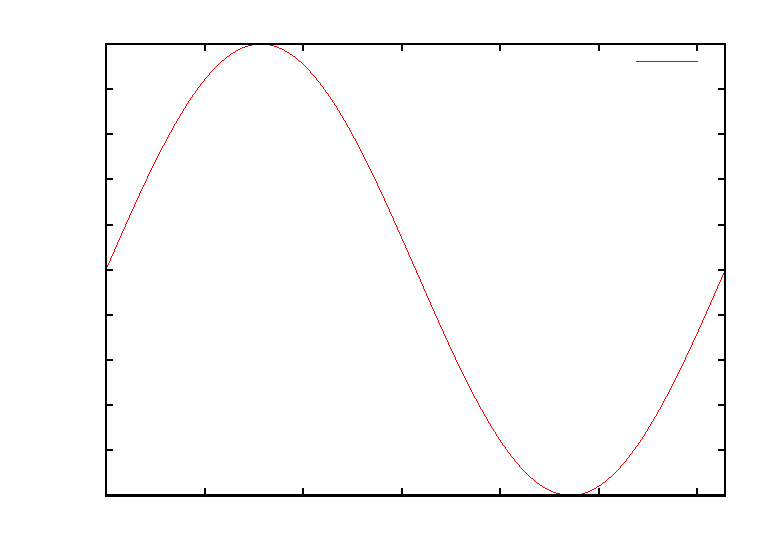
\includegraphics{sine}}%
    \gplfronttext
  \end{picture}%
\endgroup

 \end{center}
\end{figure}

Notice that the $x$-axis is labeled with integers. To get the $x$-axis labels with fractions of
$\pi$, you need to modify the \texttt{terminal} setting. In Windows, you would do this:
\begin{displaymath}
 \texttt{set terminal windows enhanced}
\end{displaymath}
In Linux you would do this:
\begin{displaymath}
 \texttt{set terminal wxt enhanced}
\end{displaymath}
You can then (provided the Symbol font is installed, which it usually is) set the $x$-axis to have
multiples of $\pi/2$ from $0$ to $2\pi$ as labels with this command (all on one line):
\begin{gather*}
 \texttt{set xtics ('0' 0,'\{/Symbol p\}/2' pi/2,'\{/Symbol p\}' pi,'3\{/Symbol p\}/2' 3*pi/2,}\\
 \texttt{'2\{/Symbol p\}' 2*pi)}
\end{gather*}
In the above example,
 to also plot the function $y=\cos\;2x + \sin\;3x$ on the same graph, put a comma after the first
 function then append the new function:
 \begin{displaymath}
  \texttt{plot \symbol{91}0:2*pi\symbol{93} sin(x), cos(2*x) + sin(3*x)}
 \end{displaymath}
By default, the $x$-axis is not shown in the graph. To display it, use this command
\emph{before} the \textbf{\path{plot}} command:
\begin{displaymath}
 \texttt{set zeroaxis}
\end{displaymath}
Also, to label the axes, use these commands:
\begin{gather*}
 \texttt{set xlabel "x"}\\\texttt{set ylabel "y"}
\end{gather*}
The default sample size for plots is $100$ units, which can result in jagged edges if the curve
is complicated. To get a smoother curve, increase the
sample size (to, say, $1000$) like this:
\begin{displaymath}
 \texttt{set samples 1000}
\end{displaymath}
Putting all this together, we get the following graph:

\begin{figure}[H]
 \begin{center}
  % GNUPLOT: LaTeX picture with Postscript
\begingroup
\footnotesize
  \makeatletter
  \providecommand\color[2][]{%
    \GenericError{(gnuplot) \space\space\space\@spaces}{%
      Package color not loaded in conjunction with
      terminal option `colourtext'%
    }{See the gnuplot documentation for explanation.%
    }{Either use 'blacktext' in gnuplot or load the package
      color.sty in LaTeX.}%
    \renewcommand\color[2][]{}%
  }%
  \providecommand\includegraphics[2][]{%
    \GenericError{(gnuplot) \space\space\space\@spaces}{%
      Package graphicx or graphics not loaded%
    }{See the gnuplot documentation for explanation.%
    }{The gnuplot epslatex terminal needs graphicx.sty or graphics.sty.}%
    \renewcommand\includegraphics[2][]{}%
  }%
  \providecommand\rotatebox[2]{#2}%
  \@ifundefined{ifGPcolor}{%
    \newif\ifGPcolor
    \GPcolortrue
  }{}%
  \@ifundefined{ifGPblacktext}{%
    \newif\ifGPblacktext
    \GPblacktexttrue
  }{}%
  % define a \g@addto@macro without @ in the name:
  \let\gplgaddtomacro\g@addto@macro
  % define empty templates for all commands taking text:
  \gdef\gplbacktext{}%
  \gdef\gplfronttext{}%
  \makeatother
  \ifGPblacktext
    % no textcolor at all
    \def\colorrgb#1{}%
    \def\colorgray#1{}%
  \else
    % gray or color?
    \ifGPcolor
      \def\colorrgb#1{\color[rgb]{#1}}%
      \def\colorgray#1{\color[gray]{#1}}%
      \expandafter\def\csname LTw\endcsname{\color{white}}%
      \expandafter\def\csname LTb\endcsname{\color{black}}%
      \expandafter\def\csname LTa\endcsname{\color{black}}%
      \expandafter\def\csname LT0\endcsname{\color[rgb]{1,0,0}}%
      \expandafter\def\csname LT1\endcsname{\color[rgb]{0,1,0}}%
      \expandafter\def\csname LT2\endcsname{\color[rgb]{0,0,1}}%
      \expandafter\def\csname LT3\endcsname{\color[rgb]{1,0,1}}%
      \expandafter\def\csname LT4\endcsname{\color[rgb]{0,1,1}}%
      \expandafter\def\csname LT5\endcsname{\color[rgb]{1,1,0}}%
      \expandafter\def\csname LT6\endcsname{\color[rgb]{0,0,0}}%
      \expandafter\def\csname LT7\endcsname{\color[rgb]{1,0.3,0}}%
      \expandafter\def\csname LT8\endcsname{\color[rgb]{0.5,0.5,0.5}}%
    \else
      % gray
      \def\colorrgb#1{\color{black}}%
      \def\colorgray#1{\color[gray]{#1}}%
      \expandafter\def\csname LTw\endcsname{\color{white}}%
      \expandafter\def\csname LTb\endcsname{\color{black}}%
      \expandafter\def\csname LTa\endcsname{\color{black}}%
      \expandafter\def\csname LT0\endcsname{\color{black}}%
      \expandafter\def\csname LT1\endcsname{\color{black}}%
      \expandafter\def\csname LT2\endcsname{\color{black}}%
      \expandafter\def\csname LT3\endcsname{\color{black}}%
      \expandafter\def\csname LT4\endcsname{\color{black}}%
      \expandafter\def\csname LT5\endcsname{\color{black}}%
      \expandafter\def\csname LT6\endcsname{\color{black}}%
      \expandafter\def\csname LT7\endcsname{\color{black}}%
      \expandafter\def\csname LT8\endcsname{\color{black}}%
    \fi
  \fi
  \setlength{\unitlength}{0.0500bp}%
  \begin{picture}(7200.00,5040.00)%
    \gplgaddtomacro\gplbacktext{%
      \csname LTb\endcsname%
      \put(946,704){\makebox(0,0)[r]{\strut{}-2}}%
      \put(946,1213){\makebox(0,0)[r]{\strut{}-1.5}}%
      \put(946,1722){\makebox(0,0)[r]{\strut{}-1}}%
      \put(946,2231){\makebox(0,0)[r]{\strut{}-0.5}}%
      \put(946,2740){\makebox(0,0)[r]{\strut{} 0}}%
      \put(946,3248){\makebox(0,0)[r]{\strut{} 0.5}}%
      \put(946,3757){\makebox(0,0)[r]{\strut{} 1}}%
      \put(946,4266){\makebox(0,0)[r]{\strut{} 1.5}}%
      \put(946,4775){\makebox(0,0)[r]{\strut{} 2}}%
      \put(1078,484){\makebox(0,0){\strut{}$0$}}%
      \put(2509,484){\makebox(0,0){\strut{}$\pi/2$}}%
      \put(3941,484){\makebox(0,0){\strut{}$\pi$}}%
      \put(5372,484){\makebox(0,0){\strut{}$3\pi/2$}}%
      \put(6803,484){\makebox(0,0){\strut{}$2\pi$}}%
      \csname LTb\endcsname%
      \put(176,2739){\rotatebox{-270}{\makebox(0,0){\strut{}$y$}}}%
      \put(3940,154){\makebox(0,0){\strut{}$x$}}%
    }%
    \gplgaddtomacro\gplfronttext{%
      \csname LTb\endcsname%
      \put(5816,4602){\makebox(0,0)[r]{\strut{}$\sin(x)$}}%
      \csname LTb\endcsname%
      \put(5816,4382){\makebox(0,0)[r]{\strut{}$\cos(2*x) + \sin(3*x)$}}%
    }%
    \gplbacktext
    \put(0,0){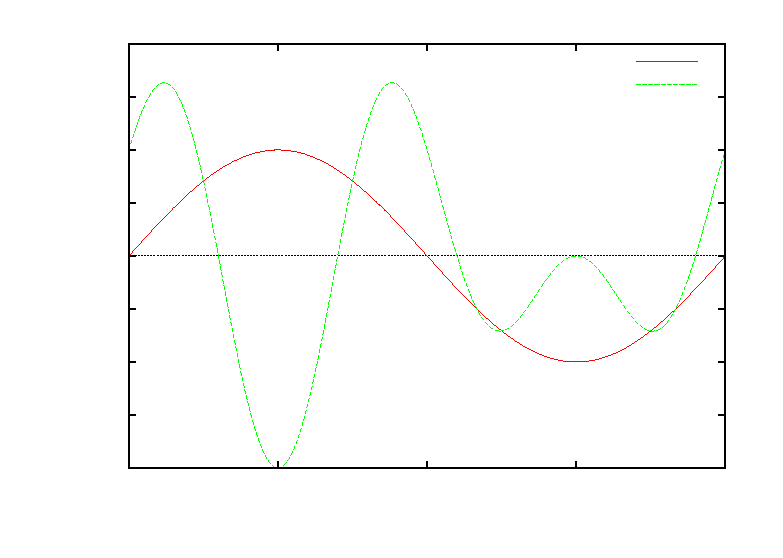
\includegraphics{tutorial}}%
    \gplfronttext
  \end{picture}%
\endgroup

 \end{center}
\end{figure}\vspace{-4mm}
\lineacross
\vspace{3mm}

\par\noindent\textbf{\textsf{PRINTING AND SAVING}}\vspace{2mm}\\
In Windows, if you are using the \texttt{windows enhanced} terminal then to print a graph from
Gnuplot click on the printer icon in the menubar of the graph's window. If you are using the
default \texttt{wxt} terminal then select \textbf{Print} near the top of the main Gnuplot window
and enter \path{png} in the \emph{Terminal type?} textfield, then hit OK to get the Print Setup
dialog.

In Windows, to save a graph, say, as a PNG file, go to the File menu on the main Gnuplot menubar,
select ``Output Device ...'', and enter \path{png} in the \emph{Terminal type?} textfield, hit OK. Then, in the
File menu again, select the ``Output ...'' option and enter a filename (say, graph.png) in the \emph{Output
filename?} textfield, hit OK. Now run your plot command again and the file will be saved in the
current directory, usually in your \texttt{My Documents} folder (it can also be found by
selecting the ``show Current Directory'' option in the File menu).\\

\par\noindent In Linux, to save the graph as a file called graph.png run the following
commands:\vspace{2mm}

\begin{tabular}{l @{}}
\texttt{set terminal png}\\
\texttt{set output 'graph.png'}
\end{tabular}\vspace{2mm}

\par\noindent and then run your plot command. There are many terminal types (which determine the output format). Run
the command \textbf{\texttt{set terminal}} to see all the possible types. In Linux, the \textbf{postscript} terminal type is
popular, since the print quality is high and there are many PostScript viewers available.
\vspace{2mm}

\par\noindent To quit Gnuplot, type \textbf{\path{quit}} at the \textbf{\path{gnuplot>}} command prompt.
